\documentclass[11pt]{article}
\usepackage{fullpage}
\usepackage{amsthm}

\usepackage{amsthm,amsmath,amsfonts,amssymb,amstext,enumitem}
\usepackage{latexsym,ifthen,url,rotating,graphicx}
\usepackage{listings}
\usepackage{tikz}
\usetikzlibrary{arrows,shapes,positioning,fit}
\usepackage{graphicx}
\usepackage[font=small,labelfont=bf]{caption}



% --- -----------------------------------------------------------------
% --- Document-specific definitions.
% --- -----------------------------------------------------------------
\lstset{
    columns=fixed,
    literate={—}{{---}}1 {…}{{...}}1
}

\newcommand{\todo}[1]{{\color{red}[TODO:{#1}]}}

\newtheorem{problem}{Problem}
\newtheorem{corollary}{Corollary}
\newtheorem{fact}{Fact}
\newtheorem{exercise}{Exercise}
\newtheorem{theorem}{Theorem}
\newtheorem{definition}{Definition}
\newtheorem{notation}{Notation}
\newtheorem{lemma}{Lemma}
\newtheorem{example}{Example}

\newcommand{\getsr}
  {{\:\stackrel{\raisebox{-2pt}{${\scriptscriptstyle \hspace{0.2em}\$}$}}
   {\leftarrow}\:}}
\newcommand{\points}[1]{\textbf{({#1} pts)}}

\newcommand{\Colon}{\ : \ }
\newcommand{\st}{\mathsf{state}}
\newcommand{\msgs}{\mathcal{M}}
\newcommand{\ctxts}{\mathcal{C}}
\newcommand{\keys}{\mathcal{K}}
\newcommand{\kg}{\mathcal{K}}
\newcommand{\enc}{E}
\newcommand{\dec}{E^{-1}}
\newcommand{\MAC}{\mathrm{MAC}}
\newcommand{\RMAC}{\mathrm{RMAC}}

\newcommand{\pk}{pk}
\newcommand{\sk}{sk}

\newcommand{\AES}{\mathsf{AES}}

\newcommand{\algorithm}[1]{\textbf{Alg} {#1}}

\newcommand{\calO}{\mathcal{O}}

\newcommand{\dlog}{\mathrm{dlog}}

\newcommand{\Adv}{\mathbf{Adv}}
\newcommand{\AdvPRF}[2]{\Adv^{\mathrm{prf}}_{#1}({#2})}
\newcommand{\AdvCPA}[2]{\Adv^{\mathrm{ind{-}cpa}}_{#1}({#2})}
\newcommand{\AdvCCA}[2]{\Adv^{\mathrm{ind{-}cca}}_{#1}({#2})}
\newcommand{\AdvKR}[2]{\Adv^{\mathrm{kr}}_{#1}({#2})}
\newcommand{\AdvCKR}[2]{\Adv^{\mathrm{ckr}}_{#1}({#2})}
\newcommand{\AdvRMR}[2]{\Adv^{\mathrm{rmr}}_{#1}({#2})}
\newcommand{\AdvCR}[2]{\Adv^{\mathrm{cr}}_{#1}({#2})}
\newcommand{\AdvUFCMA}[2]{\Adv^{\textrm{uf{-}cma}}_{#1}({#2})}
\newcommand{\AdvDL}[2]{\Adv^{\mathrm{dl}}_{#1}({#2})}

\newcommand{\Exp}{\mathbf{Exp}}
\newcommand{\ExpOW}[1]{\Exp^{\mathrm{ow}}({#1})}
\newcommand{\ExpCKR}[2]{\Exp^{\mathrm{ckr}}_{#1}({#2})}
\newcommand{\ExpRMR}[2]{\Exp^{\mathrm{rmr}}_{#1}({#2})}

\newcommand{\concat}{{\,\|\,}}
\newcommand{\xor}{\oplus}
\newcommand{\bits}{\{0,1\}}

\newcommand{\tcolh}{T^{\mathrm{col}}_h}
\newcommand{\tcolH}{T^{\mathrm{col}}_{H^2}}
\newcommand{\Hcomb}{H^{1\|2}}
\newcommand{\Hxor}{H^{1\oplus2}}

\newcommand{\EXP}{\textrm{EXP}}
\newcommand{\MODEXP}{\textrm{MOD{-}EXP}}
\newcommand{\ADD}{\textrm{ADD}}
\newcommand{\MULTIMODEXP}{\textrm{MULTI{-}MOD{-}EXP}}
\newcommand{\MUL}{\textrm{MUL}}
\newcommand{\MOD}{\textrm{MOD}}

\newcommand{\GG}{\mathbb{G}}
\newcommand{\ZZ}{\mathbb{Z}}

\newcommand{\bK}{\mathbf{K}}
\newcommand{\bM}{\mathbf{M}}
\newcommand{\bC}{\mathbf{C}}

\newcommand{\rvrange}{\mathcal{R}}
\newcommand{\rspace}{\mathcal{C}}

\newcommand{\hatalpha}{\hat{\alpha}}

\newcommand{\otp}{\mathrm{OTP}}

% --- -----------------------------------------------------------------
% --- Lecture notes formatting macros
% --- -----------------------------------------------------------------

%
% The following commands set up the lecnum (lecture number)
% counter and make various numbering schemes work relative
% to the lecture number.
%
\newcounter{lecnum}
%\renewcommand{\thepage}{\thelecnum-\arabic{page}}
\renewcommand{\thesection}{\thelecnum.\arabic{section}}
\renewcommand{\theexercise}{\thelecnum.\arabic{exercise}}
\renewcommand{\theexample}{\thelecnum.\arabic{example}}
\renewcommand{\thedefinition}{\thelecnum.\arabic{definition}}
\renewcommand{\theequation}{\thelecnum.\arabic{equation}}
\renewcommand{\thefigure}{\thelecnum.\arabic{figure}}
\renewcommand{\thefact}{\thelecnum.\arabic{fact}}
\renewcommand{\thetable}{\thelecnum.\arabic{table}}


%
% The following macro is used to generate the header.
%
\newcommand{\lecture}[2]{
   %\pagestyle{myheadings}
   %\thispagestyle{plain}
   \newpage
   \setcounter{lecnum}{#1}
   \setcounter{page}{1}
   \noindent
   \begin{center}
   \framebox{
      \vbox{\vspace{2mm}
    \hbox to 6.28in { {\bf CMSC 28400 Introduction to Cryptography
                        \hfill Autumn 2020} }
       \vspace{4mm}
       \hbox to 6.28in { {\Large \hfill #2 \hfill} }
       \vspace{2mm}
       \hbox to 6.28in { {\it Instructor: David Cash} \hfill }
      \vspace{2mm}}
   }
   \end{center}
   %\markboth{Lecture #1: #2}{Lecture #1: #2}
   \vspace*{4mm}
}





% --- -----------------------------------------------------------------
% --- The document starts here.
% --- -----------------------------------------------------------------
\begin{document}
%\lecture{**LECTURE-NUMBER**}{**DATE**}{**LECTURER**}{**SCRIBE**}
\lecture{3}{Notes \#2: Perfect Secrecy}

%\tableofcontents

%\noindent\hrulefill
%\bigskip


These notes cover our first definition of security: \emph{Perfect Secrecy},
which dates back to the work Shannon in the 1950s. The motivation for this
approach to security is to (hopefully) escape the attack-then-patch cycle that
drove classical cipher development. Abstractly, the plan is to give a
mathematical definition of ``security'' for a cipher, every bit as precise as
other definitions, and then \emph{prove} that a cipher meets this definition of
security. 

What guarantees can this plan give us, ultimately? The proof can only tell us
that attacks violating the security definition are impossible. As we will see
Several times in this course, real attacks may work without
violating the definition; They instead violate some underlying assumption about
how the definition corresponds to reality. (An extreme example could be an
attacker who steals your laptop and gets your key. Clearly all bets are off,
even if you had a nice proof.)

Below we start with the security definition, and then prove the One-Time-Pad
achieves this definition. In the next set of notes we'll discuss limitations of
this definition, and generalize it to something more practical.

\section{How to Evaluate the Security of Ciphers?}

First let's recall the definition of a cipher from the previous notes,
for use below.
\begin{definition}
    Let $\keys,\msgs,\ctxts$ be non-empty sets. A function
    \[
        \enc : \keys\times\msgs \to \ctxts
    \]
    is called a \emph{cipher with key-space $\keys$, message-space
    $\msgs$, and ciphertext-space $\ctxts$} if for every $K\in\keys$,
    the function $\enc(K,\cdot)$ is one-to-one.

    For such a cipher, we define 
    \[
        \dec: \keys\times\ctxts \to\msgs
    \]
    by letting $\dec(K,\cdot)$ be the inverse of $\enc(K,\cdot)$ for
    each $K\in\keys$. (More precisely, $\dec(k,c)$ is only defined when
    there exists $m\in\msgs$ such that $\enc(k,m)=c$.)
\end{definition}

Suppose $E$ is a cipher. What does it mean for $E$ to be ``secure''? We could come
up with list of attacks that it should resist. We could say that $E$ should
resist single-character frequency analysis, or bigram frequency analysis, or
more and more clever attacks as we learn about them.  Or, we could ask
more abstractly that ``no one should be able to recover an encrypted message'',
or even ``no one should be able to recover any part of an encrypted message'',
though as a cipher designer it would be hard to interpret such a goal. Someone
could convince us that we hadn't achieved those goals by presenting an attack,
but how could someone possibly convince us that they \emph{had} achieved the
such goals? 

The approach to answering this question taken in the next subsection is to give
a mathematical definition of security which compresses a long list of
security properties into one simple requirement. If one deems the
definition suitable for an application, then the proof is enough to convince
you that a cipher ``is secure.''

Before we dive in, it is worth noting that the approach of enumerating possible
attacks is fundamental to modern cryptography. As we will see later, we can't
give definitions and proofs for everything. But our philosophy will be to use
definitions and proofs as a tool to help drive our cipher design and limit
security risk.

\subsection{The Definition of Perfect Secrecy}

Let's just lay the definition out and then discuss it, first at a purely
syntactic level, then at an intuitive level.
\begin{definition}Let $\enc : \keys\times\msgs \to \ctxts$ be a cipher and
    $\bK$ be a uniform random variable on $\keys$.  We say that $\enc$ is
    \emph{perfectly secret} if for all $m_1,m_2\in\msgs$, and $c\in\ctxts$,
    \[
        \Pr[\enc(\bK,m_0) = c] = \Pr[\enc(\bK,m_1) = c].
    \]
\end{definition}
In the probabilities, $\bK$ is the only random variable. So for instance
the left probability is determined by how often $m_0$ will encrypt to
$c$ with a randomly-chosen key; The other probability is the same except
with $m_1$. But in both probabilities, $m_0,m_1$, and $c$ are \emph{fixed}
and not random.

Intuitively, this definition says that which message you are encrypting
should not affect the distribution of the ciphertext you get. This is great
for security, because it means an attacker looking at the ciphertext gets
``no information'' about what the message was.

\begin{exercise}
    Show that the substitution cipher is not perfectly secret.  (Hint:
    Considering a ciphertext like $c=\mathtt{AA}$ makes this more clear, but
    any ciphertext will work.)
\end{exercise}

We can try to understand this definition by giving an equivalent version.
The following definition is somewhat more complicated technically, but may
be more clear. It is equivalent to perfectly secrecy, in the sense that
any cipher $E$ that is perfectly secret meets this definition, and vice versa.
\begin{definition} 
    Let $\enc : \keys\times\msgs \to \ctxts$ be a cipher and $\bK$ be a uniform
    random variable on $\keys$.  We say that $\enc$ has \emph{independent
    ciphertexts} if for all random variables $\bM$ on $\msgs$ independent of
    $\bK$, we have that the random variable $\bC = \enc(\bK,\bM)$ is
    independent of $\bM$.
\end{definition}
Here we use a random variable $\bM$ to model picking a message
in some application-dependent way (or to model the distribution of the message
given an attacker's knowledge). For instance, if an attacker knows you
sending a payment response to a website, it might know every character of your
message except your credit card number. In that case $\bM$ could be a fixed
request but with random digits for the credit card number.

Note also in the definition that $\bC$ is another random variable defined as a
function of $\bK$ and $\bM$. The probability notes review the underlying
foundations of what this means mathematically (though, as the notes mention, we
are operating without explicitly saying what the sample space is, and will
continue to do so in later definitions).


\begin{theorem}
    A cipher $\enc : \keys\times\msgs \to \ctxts$ is perfectly secret
    if and only if it has independent ciphertexts.
\end{theorem}

\begin{exercise}
    Prove this theorem. (Hint: There are two directions. You will need
    to look up the precise definition of independent random variables
    if you are unsure how to proceed rigorously.)
\end{exercise}

\section{The One-Time Pad is Perfectly Secret}

We now carry out the second step in our plan: Constructing a cipher and proving
that it is perfectly secret. We'll use the last of our historical ciphers, the
one-time pad.  Concretely, for each integer $n\geq 1$, define a cipher
$\otp_n : \bits^n\times\bits^n \to \bits^n$ by
\[
    \otp_n(k,m) = k \oplus m.
\]
These ciphers are perfectly secret, as we now prove.
\begin{theorem}
    For every integer $n\geq 1$, the cipher $\otp_n$ is perfectly secret.
\end{theorem}
\begin{proof} We use the original definition, so we have to show that for every
    $m_0,m_1\in\bits^n$ and $c\in\bits^n$,
    \[
        \Pr[\enc(\bK,m_0) = c] = \Pr[\enc(\bK,m_1) = c],
    \]
    where $\bK$ is uniform on $\bits^n$.  We will do even better, and show that
    for every $m\in\bits^n$ and $c\in\bits^n$,
    \[
        \Pr[\enc(\bK,m) = c] = 2^{-n}, 
    \]
        which will imply what we need (if the probabilities are all $2^{-n}$ no
        matter what $m$ and $c$ are, then certainly the probabilities above are
        equal). This follows because
    \[
        \Pr[\enc(\bK,m) = c] = \Pr[\bK\oplus m=c] = \Pr[\bK=c\oplus m] = 2^{-n}.
    \]
    The first two equalities hold because $\enc(\bK,m)=c$, $\bK\oplus m = c$,
    and $\bK=c\oplus m$ are all the \emph{same event} (one happens if and only
    if the others happen; it looks like simple manipulation of the equations,
    but it is formally justified by them representing the same event). The last
    equality holds because $\bK$ is uniform and $c\oplus m$ is just a fixed
    element of $\bits^n$.
\end{proof}
As short as it is, this proof might be tricky if you are not used to
manipulating random variables. It is worth referring back to the probability
background if you found the equalities in the proof difficult to verify.

This theorem explains why we needed to have multiple encryptions under the same
key in order to break a one-time pad cipher: If we only had one ciphertext,
then we'd effectively have only a random string, independent of the message.
But once more than one ciphertext with the same key is available, attacks like
crib-dragging are effective.

\begin{exercise}
    Define a version of the Vigen\`{e}re cipher with an $n$-letter
    key working only on ciphertexts of $n$ letters. Show that this
    cipher is perfectly secret.
\end{exercise}

\begin{exercise}
    Define a cipher $E:\bits\times\{0,1,2\}\to\{0,1,2\}$ by $E(k,m) = k+m\bmod
    3$. Show directly that $E$ is not perfectly secret. (This will also be a
    consequence of a later theorem.)
\end{exercise}


\iffalse
\section{Perfectly Secret Ciphers Must Have $|\keys| \geq |\msgs|$}

The $n$-bit one-time pad has key as long as the messages, which is inconvenient
when messages are long. The following theorem shows this is in some sense
unavoidable when one insists of having a perfectly secret cipher.
\begin{theorem}
    A cipher $\enc : \keys\times\msgs \to \ctxts$ is perfectly secret
    if and only if it has independent ciphertexts.
\end{theorem}
\begin{proof}
    We prove the contrapositive, meaning we show that if $|\keys| < |\msgs|$,
    then $E$ is not perfectly secret. In order to show $E$ is not perfectly
    secret, we find some $m_0,m_1\in\msgs$ and $c\in\ctxts$ such that
    \begin{align}\label{neqprob}
        \Pr[\enc(\bK,m_0) = c] \neq \Pr[\enc(\bK,m_1) = c],
    \end{align}
    where $\bK$ is uniform on $\keys$.

    We start by taking $c\in\ctxts$ to be an arbitrary element of the image of
    $E$ (so, we know that $E(k,m)=c$ for some $k\in\keys,m\in\msgs$, but we
    don't care how its picked beyond that).

    Define the set $X$ of ``all possible decryptions of $c$'' as
    \[
        X = \{E^{-1}(k,c) \ | \ k\in\keys \}.
    \]
    Notice that $|X| \leq |\keys|$, because at most one element is added to $X$
    per element of $\keys$ (it might be less because we might add the same
    element twice). By our choice of $c$ we also have that $X$ is non-empty;
    pick some arbitrary $m_1\in X$.

    Since $|X| \leq |\keys|$, and we assumed $|\keys| < |\msgs|$, we have
    $|X| \leq |\msgs|$. Therefore $X$ does not contain all of $\msgs$, and
    can choose some $m_0 \in \msgs$ that is not in $X$.
    The following diagram shows the relationship between $c,m_1$ and $m_0$.
    \begin{center}
        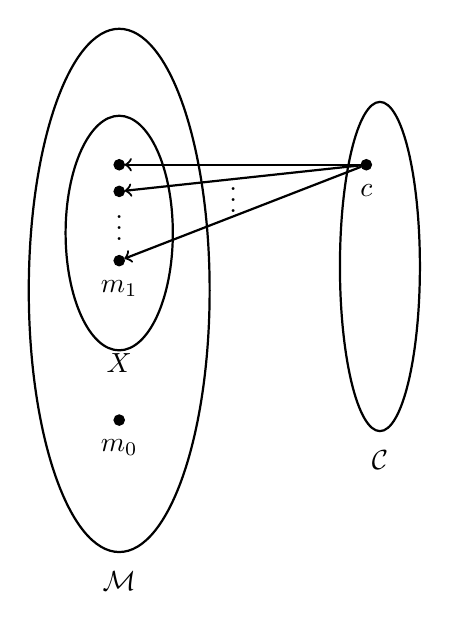
\begin{tikzpicture}
            \tikzstyle{connect}=[circle, draw, thin,fill=black, scale=0.4]
            \tikzstyle{every path}=[thick]
            \tikzstyle{rotor}=[very thick, rounded corners]
            \tikzstyle{input}=[circle,draw,scale=.7]
            \tikzstyle{internalwire}=[thick,darkgray]

            \node[connect] (m1) {};
            \node[connect, below=.2cm of m1] (m2) {};
            \node[below=-.1cm of m2] (dots) {$\vdots$};
            \node[connect, below=.05cm of dots] (m3) {};
            \node[below=.05cm of m3] (m3label) {$m_1$};
            \node[shape=ellipse,draw,fit={(m1) (m3label)}] (X) {};
            \node[below=-.1cm of X] (Xlabel) {$X$};

            \node[connect, below=.4cm of Xlabel] (m0) {};
            \node[below=.05cm of m0] (m0label) {$m_0$};

            \node[shape=ellipse,draw,minimum width=1.5cm,fit={(X) (m0label)}] (msgs) {};
            \node[below=.1cm of msgs] {$\msgs$};

            \node[connect, right=3cm of m1] (c) {};
            \node[below=.05cm of c] (clabel) {$c$};
            \node[right=3cm of Xlabel] (cinvis) {};
            \node[shape=ellipse,draw,minimum width=1cm,fit={(c) (cinvis)}] (ctxts) {};
            \node[below=.1cm of ctxts] {$\ctxts$};

            \draw [->] (c) -- (m1);
            \draw [->] (c) -- (m2);
            \node[right=1.2cm of m2] {$\vdots$};
            \draw [->] (c) -- (m3);

        \end{tikzpicture}
    \end{center}
    We have chosen our $m_0,m_1$, and $c$. It remains to verify that
    (\ref{neqprob}) holds. This follows by two observations:
    \begin{itemize}
        \item $\Pr[E(\bK,m_0)=c] = 0$, because there is no key $k$ such
            that $E(k,m_0)=c$.
        \item $\Pr[E(\bK,m_1)=c] \geq 1/|\keys| > 0$, because there
            is at least one key $k$ such that $E(k,m_1)=c$.
    \end{itemize}
    This shows the probabilities are not equal and completes the proof.
\end{proof}
\fi
\end{document}


